% =====================================================================
%  Chapter 1 — What a \idxw{Catalogue} Entry Cannot Tell You
% =====================================================================

\chapter{What a Catalogue Entry Cannot Tell You}
\label{ch:catalogue-entry}

A near-Earth object\idx{Near-Earth object} enters the record as a line. The line carries a
designation, a set of orbital elements, an absolute magnitude\idx{Absolute magnitude}, a geometrical
albedo\idx{Albedo} where one has been measured, and a probability of impact that is usually
negligible. It is the most efficient kind of scientific record there is, and
for the job the catalogue\idx{Catalogue} was built to do --- telling the Solar System's
near-Earth population from the rest of the Solar System --- it is excellent.

It is a poor record for the job the planetary-defence community needs done.
A catalogue\idx{Catalogue} entry does not contain a size, a mass, a shape, a spin state, a
bulk density, a rotation axis, or a thermal inertia. It does not contain an
energy. It contains, at most, an absolute magnitude\idx{Absolute magnitude}, which is a statement
about the object's brightness and which the catalogue\idx{Catalogue} itself records as
uncertain. Everything a defender would want to know about what would happen
on impact has to be inferred on the side, from models whose assumptions are
seldom written down and whose errors are seldom carried forward.

\section{The population, as it actually stands}

The scale of the problem is worth stating first, because it is not what most
people assume. The NASA Center for Near Earth Object Studies publishes a
cumulative discovery series, and as of 22 November 2026 it contained
43,212 known near-Earth objects, of which 11,725 were larger than about
140~metres and 883 were larger than about one kilometre. The catalogue is
growing at roughly three thousand objects a year across all sizes, but the
growth is not uniform: the sub-140-metre population is still arriving at
thousands a year, while the 140-metre class has slowed to a few hundred and
the kilometre class to two or three annually.

\begin{figure}[!htbp]
\centering
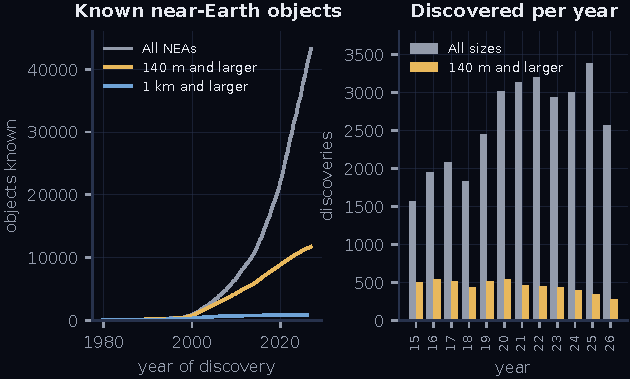
\includegraphics[width=\textwidth]{../figures/fig_catalogue.pdf}
\caption{The cumulative catalogue of known near-Earth objects by size class,
and the annual discovery rate. The kilometre class is essentially complete;
the 140-metre class is closing; the sub-140-metre population is still
arriving at three thousand a year. Source: NASA CNEOS discovery statistics,
data current 22 November 2026.}
\label{fig:catalogue}
\end{figure}

The asymmetry in \figref{fig:catalogue} is the first thing the reader should
take from it. The catalogue is nearly complete at the top and still growing at
the bottom, which means that the objects that can destroy a city are already,
for the most part, known. The problem is not that we are failing to find the
dangerous ones. The problem is that we know they are there and we do not
know what they are.

\section{What is missing, and why each thing is missing}

The missing quantities are missing for different reasons, and the differences
matter, because a measurement that is merely difficult is a different
procurement problem from a measurement that is impossible.

The \emph{size} is missing because the object is unresolved. Its brightness is
recorded and its size is not, because converting one to the other requires an
albedo\idx{Albedo}, and the albedo\idx{Albedo} is a function of composition, and composition has to be
measured. This is the degeneracy that Chapter 6 takes apart in full. The
\emph{mass} is missing because mass requires either a dynamical measurement
--- an orbit disturbed by the object itself, which for a small body means a
close approach to something massive --- or a volume and a density, and the
density is itself uncertain by a factor of about three between a rubble pile
and a monolith.

The \emph{shape} is missing because resolving a sixty-metre object at a
hundredth of an astronomical unit demands either proximity or an aperture that
nobody owns. The \emph{spin state} is missing for a different reason: it is
the easiest of the missing quantities to obtain, because a lightcurve is
cheap, and it is still missing for most objects simply because nobody has
pointed a telescope at them for long enough.

\section{Two chains through one measurement}

What follows from this inventory is the structural observation that organises
the rest of the book. The two things a defender needs are an energy and a
probability. Each of those is computed from the same physical inputs, by
chains that run in different directions but share their first link.

\begin{table}[!htbp]
\centering
\footnotesize
\caption{The two chains through the shape measurement. The right column is the
measurement that closes each link.}
\label{tab:chains}
\begin{tabularx}{\textwidth}{@{}P{0.64in}P{1.08in}YY@{}}
\toprule
\rowcolor{panel}
\textbf{Chain} & \textbf{Link} & \textbf{What limits it} & \textbf{What closes it} \\
\midrule
Accounting & Shape to volume & unknown scale & resolved imaging, or thermal flux \\
\rowcolor{panel}
 & Volume to mass & rubble pile against monolith & radar, flyby, thermal inertia \\
 & Mass to energy & \(\delta\ln E = 3\,\delta\ln D + \delta\ln \rho\) &
 diameter\idx{Diameter} to about 14 per cent \\
\rowcolor{panel}
 & Energy to hazard class & the Torino scale boundaries &
 diameter\idx{Diameter} and density together \\
Probability & Shape to YORP torque & surface normals and roughness &
 resolved shape \\
\rowcolor{panel}
 & Torque to spin state & pole known only to tens of degrees &
 lightcurve with a resolved shape \\
 & Spin state to Yarkovsky drift & thermal inertia unknown by an order of
 magnitude & thermal spectroscopy \\
\rowcolor{panel}
 & Drift to keyhole & along-track position at the horizon &
 everything above \\
\bottomrule
\end{tabularx}
\end{table}

\tabref{tab:chains} is the book's whole argument in one table. The
\emph{accounting} chain runs shape to volume to mass to energy to hazard
class. The \emph{probability} chain runs shape to YORP torque to spin state to
Yarkovsky drift to along-track displacement to keyhole. They are ordinarily
treated as separate problems, because they are owned by different programmes:
one is a sizing problem and the other is an orbit-determination problem. But
the first link of both is the same observation, made by the same instrument,
on the same body, at the same time. A resolved image of a rotating asteroid
does both jobs.

\section{Shape as the centre of gravity}

This is why the book is organised around shape rather than around ranging,
despite the owner's original instinct toward a ranging beam to Earth, and
despite the fact that ranging is the more familiar planetary-defence
activity. A range measurement tells you how far away an object is. A shape
measurement tells you how far away it is \emph{and} what it is made of, and
it feeds two chains instead of one.

There is a second reason, and it is quantitative rather than editorial. The
probability chain's sensitivity to physical error is not uniform across
horizons: at seven years the astrometric term dominates the impact
probability by three orders of magnitude, and at thirty years the physical
term dominates it by two or three. The measurement that matters is therefore
not the one that is always needed but the one that is needed at the horizon
where the physics has overtaken the astrometry. Chapter 14 works that out
with published numbers, and Chapter 30 turns it into the rule that decides
which platform to use.

\begin{keytakeaways}
\item The catalogue holds 43,212 near-Earth objects, 11,725 of them larger
than about 140 metres, and the dangerous ones are already mostly found.
\item A catalogue entry carries no size, mass, shape, spin state or density,
and each is missing for a different reason.
\item The accounting chain and the probability chain share their first link:
the resolved shape.
\item Because the physical term only overtakes the astrometric term at long
horizons, the measurement is needed selectively rather than routinely.
\end{keytakeaways}
